\documentclass[10pt,twoside,slovak,a4paper]{article}

\usepackage[slovak]{babel}
\usepackage[IL2]{fontenc}
\usepackage[utf8]{inputenc}
\usepackage{graphicx}
\usepackage{url} 
\usepackage{hyperref}
\usepackage{cite}

\graphicspath{ {./images/} }

\pagestyle{headings}

\title{Detekcia podvádzania v online multiplayer hrách\thanks{Semestrálny projekt v predmete Métody inžinierskej práce, akademický rok 2022/2023, vedenie: Igor Stupavský}}

\author{Tomáš Drga\\[2pt]
	{\small Slovenská technická univerzita v Bratislave}\\
	{\small Fakulta informatiky a informačných technológií}\\
	{\small \texttt{xdrga@stuba.sk}}
	}

\date{\small 10.10.2022}



\begin{document}

\maketitle

\begin{abstract}
Ako zvolenú tému som si vybral detekovanie podvodov v onlinech hrách. O túto tématiku som sa zaujímal už aj v minulosti, a tak mi prišla aj ako vhodná téma pre moju semestrálnu prácu v predmete Métody inžinierskej práce. V tomto článku sa dozviete ako sa doposiaľ detekovali podvody v online hrách, a taktiež ako sa to zmenilo s príchodom nových technológií.
\end{abstract}


\section{Úvod}\label{uxfavod}

Podvody vo videohrách sú stále častejšie medzi bežnými hráčmi, rovnako
aj medzi profesionálnymi hráčmi, čo ovplyvňuje zážitok pre všetkých
hráčov. 

Cheaty sú často bežne a~ľahko dostupné. Ak by len 6\% hráčov
používalo cheaty pri videohrách, pravdepodobnosť že sa stretnete
s~cheaterom pri hre 5 na 5 je 42,7\%\cite{pravdepodobnost}. 

Ak majú hráči podozrenie, že ostatní hráči pri hraní podvádzajú, často sa presunú k~hraní iných hier alebo začnú sami podvádzať, čím sa vytvorí nekonečný kolobeh.


\section{Diagram aktivity}\label{uxfavod}

Diagram aktivity je jeden z UML diagramov, ktorý opisuje správanie. Tento diagram sa používa na modelovanie procedurálnej logiky, procesov a zachytenia workflow.

Sekvenciu jednotlivých krokov v diagrame aktivít určuje riadiaci tok.

Každý proces v diagrame aktivity je reprezentovaný sekvenciou jednotlivých krokov, ktoré sú v modeli zakreslené ako:

akcie – atomické ďalej nedeliteľné kroky


vnorené aktivity – volanie iných aktivít.

\begin{figure}[h]
    \centering
    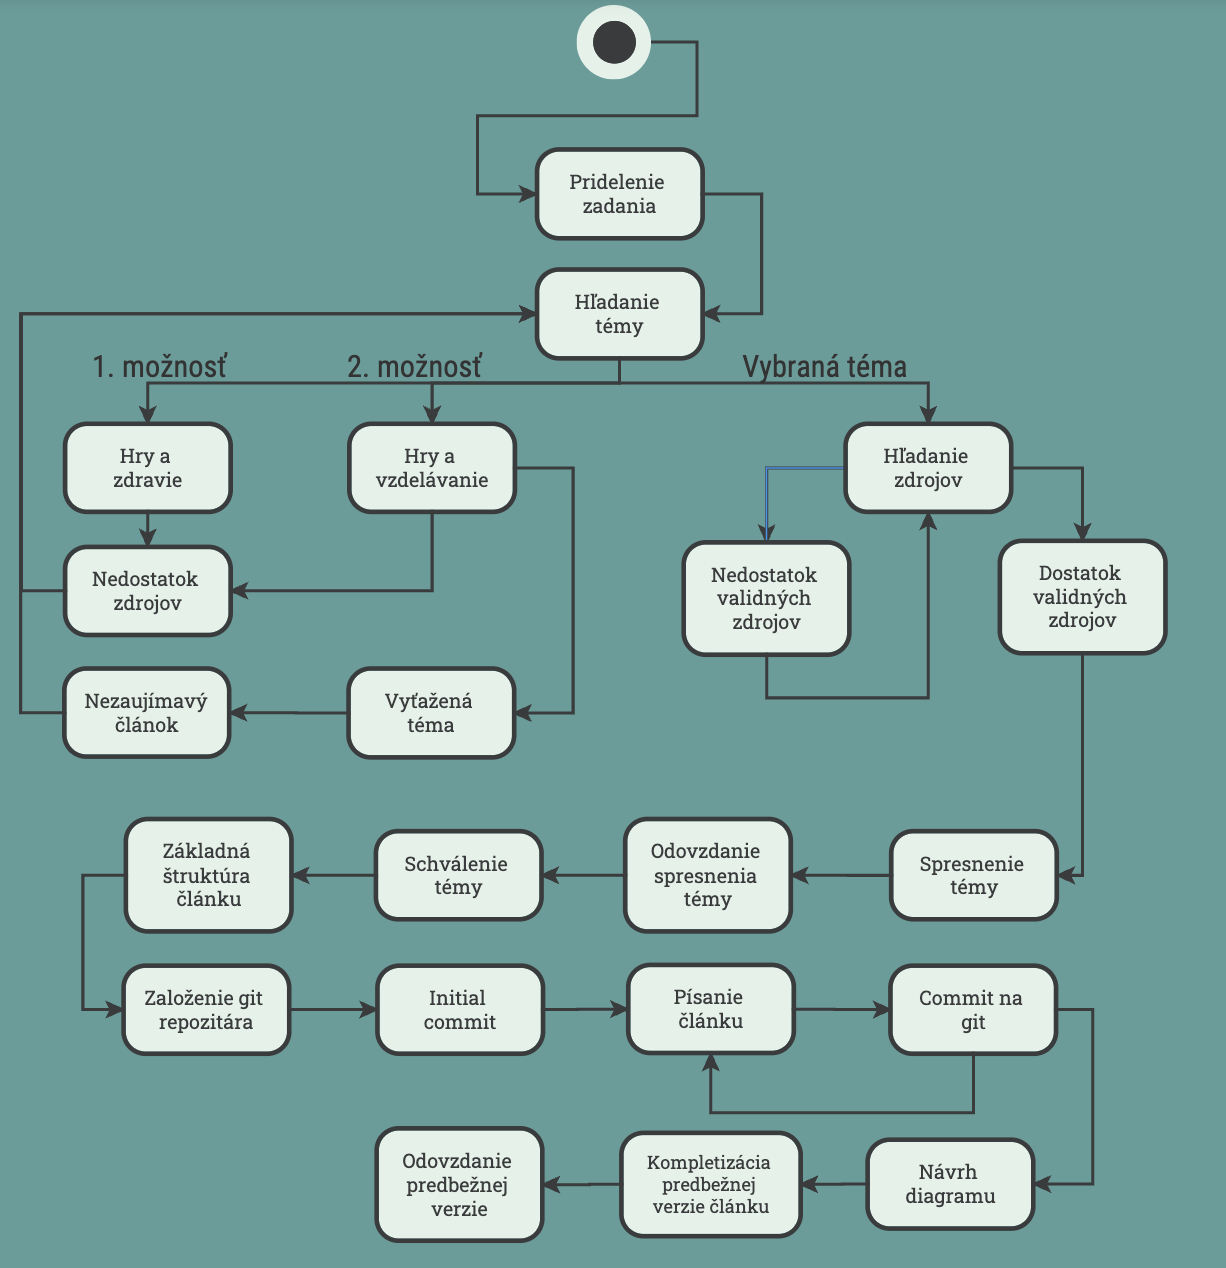
\includegraphics[width=1\textwidth]{diagram.png}
    \caption{Diagram aktivity pre písanie predbežnej verzie článku}
    \label{fig:mesh1}
\end{figure}

\section{História}

V tejto sekcií si povieme ako sa používal anticheat doteraz a prečo prišiel čas na zmenu. 

Anticheat fungoval pomerne jednoducho nakoľko nebolo možné overiť či hráč naozaj podvádza v dôsledku nedostatku informácií zo servera. Nedostatok informacií si môžeme spojiť so zabezpečením hry. No keďže nie je dostatok informácií na odhalenie podvodov museli herné spoločnsoti prísť s novými riešeniami nakoľko prichádzali o veľké množstvo peňazí a hry strácali na popularite.

\hypertarget{typy-cheatov}{%
\section{\texorpdfstring{Typy cheatov
}{Typy cheatov }}\label{typy-cheatov}}

Pri streleckých videohrách sa môžeme stretnúť rôznymi typmi použitia
cheatov, ktoré rôzne ovplyvňujú priebeh hry u~všetkých hráčov.

\hypertarget{mechanickuxe1-asistencia}{%
\subsection{Mechanická asistencia}\label{mechanickuxe1-asistencia}}

Najčastejším cheatom pri hraní streleckých hier je automatické
zameriavanie zbrane na hlavu protivníka. Tento typ podvádzania výrazne
zvýhodňuje hráčov, oproti tým, ktorí cheaty nepoužívajú.\cite{aim}

\hypertarget{asistencia-vedomostuxed-hruxe1ux10da}{%
\subsection{Asistencia vedomostí
hráča}\label{asistencia-vedomostuxed-hruxe1ux10da}}

Druhým častým podvodom v~hrách je získanie iných vedomostí oproti
ostatným hráčom. To sa odráža od princípu streleckých hier a~to je
eliminovať súpera. Tento druh cheatov dáva hráčom informácie
najčastejšie o presnej~polohe ostatných hráčov na mapách. Tieto cheaty
môžu mať rôzne podoby. 

Tento typ cheatov sa nazýva aj vizuálny hack,
alebo wallhack. To upravuje steny a~predmety vo videohrách a~ich
priehľadnosť, čím hráč môže vidieť ukrytého súpera. Taktiež je možná
úprava mapy, kde vidieť farebné odlíšenie spoluhráčov a~súperov.\cite{wallhack}

\hypertarget{asistencia-vedomostuxed-hruxe1ux10da}{%
\subsection{Motivácia pre tvorbu anticheatu}\label{asistencia-vedomostuxed-hruxe1ux10da}}
Aby sa cheatovaniu, tým pádom strate hráčov zabránilo, developeri
vytvárajú anti-cheat softvéry na detekciu cheatov ešte predtým ako sa
dostanú do hry.

Techniky data miningu analyzujú informácie v~dátach zariadenia na
zistenie cheatovacích softvérov. Táto technika však nie je ohľaduplná
k~súkromiu hráčov, nakoľko má anti-cheat softvér prístup ku všetkým
dátam hráča. Súkromnejšie techniky zistenia cheatov v~hrách momentálne
nie sú dostupné.



\bibliography{literature}
\bibliographystyle{ieeetr}
\end{document}